\documentclass[12pt, titlepage]{article}

\usepackage{fullpage}
\usepackage[round]{natbib}
\usepackage{multirow}
\usepackage{booktabs}
\usepackage{tabularx}
\usepackage{graphicx}
\usepackage{float}
\usepackage{hyperref}
\hypersetup{
    colorlinks,
    citecolor=blue,
    filecolor=black,
    linkcolor=red,
    urlcolor=blue
}

%% Comments

\usepackage{color}

\newif\ifcomments\commentstrue %displays comments
\newif\ifcomments\commentsfalse %so that comments do not display

\ifcomments
\newcommand{\authornote}[3]{\textcolor{#1}{[#3 ---#2]}}
\newcommand{\todo}[1]{\textcolor{red}{[TODO: #1]}}
\else
\newcommand{\authornote}[3]{}
\newcommand{\todo}[1]{}
\fi

\newcommand{\wss}[1]{\authornote{blue}{SS}{#1}} 
\newcommand{\plt}[1]{\authornote{magenta}{TPLT}{#1}} %For explanation of the template
\newcommand{\an}[1]{\authornote{cyan}{Author}{#1}}

%% Common Parts

\newcommand{\progname}{Sayyara} % PUT YOUR PROGRAM NAME HERE
\newcommand{\authname}{Team 31
\\ SFWRENG 4G06
\\ Christopher Andrade
\\ Alyssa Tunney
\\ Kai Zhu
\\ Ethan Vince-Budan
\\ Collin Kan
\\ Harsh Gupta} % AUTHOR NAMES                  

\usepackage{hyperref}
    \hypersetup{colorlinks=true, linkcolor=blue, citecolor=blue, filecolor=blue,
                urlcolor=blue, unicode=false}
    \urlstyle{same}

\newcounter{acnum}
\newcommand{\actheacnum}{AC\theacnum}
\newcommand{\acref}[1]{AC\ref{#1}}

\newcounter{ucnum}
\newcommand{\uctheucnum}{UC\theucnum}
\newcommand{\uref}[1]{UC\ref{#1}}

\newcounter{fenum}
\newcommand{\fethefenum}{FE\thefenum}
\newcommand{\feref}[1]{FE\ref{#1}}
\newcommand{\femoduledef}[1]{\refstepcounter{fenum} \hyperref[fe#1def]{\fethefenum}: #1 \label{fe#1}}
\newcommand{\labelfedef}[1]{\label{fe#1def}}

\newcounter{benum}
\newcommand{\bethebenum}{BE\thebenum}
\newcommand{\beref}[1]{BE\ref{#1}}
\newcommand{\bemoduledef}[1]{\refstepcounter{benum} \hyperref[be#1def]{\bethebenum}: #1 \label{be#1}}
\newcommand{\labelbedef}[1]{\label{be#1def}}

\begin{document}

\title{Module Guide for \progname{}} 
\author{\authname}
\date{\today}

\maketitle

\pagenumbering{roman}

\section*{Revision History}

\begin{table}[H]
    \begin{tabularx}{\textwidth}{p{3cm}p{2cm}X}
        \toprule {\bf Date} & {\bf Version} & {\bf Notes}\\
        \midrule
        Jan. 18, 2023 & Rev 0 & Revision 0\\
        April 5, 2023 & Rev 1 & Revision 1 \\
        \bottomrule
    \end{tabularx}
    \caption{Revision History}
\end{table}

\newpage

\section*{Reference Material}

This section records information for easy reference.

\subsection*{Abbreviations and Acronyms}

\renewcommand{\arraystretch}{1.2}
\begin{table}[H]
    \centering
    \begin{tabular}{l l} 
        \toprule		
        \textbf{symbol} & \textbf{description}\\
        \midrule 
        AC & Anticipated Change\\
        GUI & Graphical User Interface \\
        M & Module \\
        MG & Module Guide \\
        OS & Operating System \\
        R & Requirement\\
        SC & Scientific Computing \\
        SRS & Software Requirements Specification\\
        \progname & Explanation of program name\\
        UC & Unlikely Change \\
        \bottomrule
    \end{tabular}
    \caption{Abbreviations and Acronyms}
\end{table}
    
\newpage

\tableofcontents

\listoftables

\listoffigures

\newpage

\section{Introduction}
% Collin

Decomposing a system into modules is a commonly accepted approach to developing software.  A module is a work assignment for a programmer or programming
team.  We advocate a decomposition based on the principle of information hiding. This principle supports design for change, because the ``secrets'' that
each module hides represent likely future changes.  Design for change is valuable in SC, where modifications are frequent, especially during initial
development as the solution space is explored. \\

\noindent Our design follows the rules laid out by Parnes et al., as follows:
\begin{itemize}
\item System details that are likely to change independently should be the
  secrets of separate modules.
\item Each data structure is implemented in only one module.
\item Any other program that requires information stored in a module's data
  structures must obtain it by calling access programs belonging to that module.
\end{itemize}

\noindent After completing the first stage of the design, the Software Requirements
Specification (SRS), the Module Guide (MG) is developed. The MG
specifies the modular structure of the system and is intended to allow both
designers and maintainers to easily identify the parts of the software.  The
potential readers of this document are as follows:

\begin{itemize}
\item New project members: This document can be a guide for a new project member
  to easily understand the overall structure and quickly find the
  relevant modules they are searching for.
\item Maintainers: The hierarchical structure of the module guide improves the
  maintainers' understanding when they need to make changes to the system. It is
  important for a maintainer to update the relevant sections of the document
  after changes have been made.
\item Designers: Once the module guide has been written, it can be used to
  check for consistency, feasibility, and flexibility. Designers can verify the
  system in various ways, such as consistency among modules, feasibility of the
  decomposition, and flexibility of the design.
\end{itemize}

\noindent The rest of the document is organized as follows. Section
\ref{SecChange} lists the anticipated and unlikely changes of the software
requirements. Section \ref{SecMH} summarizes the module decomposition that
was constructed according to the likely changes. Section \ref{SecConnection}
specifies the connections between the software requirements and the
modules. Section \ref{SecMD} gives a detailed description of the
modules. Section \ref{SecTM} includes two traceability matrices. One checks
the completeness of the design against the requirements provided in the SRS. The
other shows the relation between anticipated changes and the modules. Section
\ref{SecUse} describes the use relation between modules.

\section{Anticipated and Unlikely Changes} \label{SecChange}

This section lists possible changes to the system. According to the likeliness
of the change, the possible changes are classified into two
categories. Anticipated changes are listed in Section \ref{SecAchange}, and
unlikely changes are listed in Section \ref{SecUchange}.

\subsection{Anticipated Changes} \label{SecAchange}

Anticipated changes are the source of the information that is to be hidden
inside the modules. Ideally, changing one of the anticipated changes will only
require changing the one module that hides the associated decision. The approach
adapted here is called design for change.

\begin{description}
\item[\refstepcounter{acnum} \actheacnum \label{acDevice}:] The specific
  devices that users access the frontend from.
\item[\refstepcounter{acnum} \actheacnum \label{acUsers}:] The number of total and concurrent users
\item[\refstepcounter{acnum} \actheacnum \label{acStorage}:] The database storage required to accommodate total and concurrent users.
\item[\refstepcounter{acnum} \actheacnum \label{acBandwidth}:] The network bandwidth required to accommodate total and concurrent users.
%\item[\refstepcounter{acnum} \actheacnum \label{acAttributes}:] The number and type of attributes in each data model.
\item[\refstepcounter{acnum} \actheacnum \label{acGUI}:] The GUI display resolution and styling.
\item[\refstepcounter{acnum} \actheacnum \label{acAuth}:] Access control methods such as openID authentication support.
\item[\refstepcounter{acnum} \actheacnum \label{acScheduling}:] The specific level of time granularity for appointment scheduling.
\item[\refstepcounter{acnum} \actheacnum \label{acNotification}:] The method notification delivery (e.g. email, real-time messaging, etc)
\item[\refstepcounter{acnum} \actheacnum \label{acHardware}:] The hardware that the backend is hosted on.
\end{description}

\subsection{Unlikely Changes} \label{SecUchange}

The module design should be as general as possible. However, a general system is
more complex. Sometimes this complexity is not necessary. Fixing some design
decisions at the system architecture stage can simplify the software design. If
these decision should later need to be changed, then many parts of the design
will potentially need to be modified. Hence, it is not intended that these
decisions will be changed.

\begin{description}
\item[\refstepcounter{ucnum} \uctheucnum \label{ucLang}:] Software compatibility for backend (Python, Django) and frontend (Typescript, NextJS)
\item[\refstepcounter{ucnum} \uctheucnum \label{ucIO}:]  Input methods (cursor, keyboard, touch).
\item[\refstepcounter{ucnum} \uctheucnum \label{ucShops}:] The system will always be able to provide a list of all registered repair shops.
\item[\refstepcounter{ucnum} \uctheucnum \label{ucAuth}:] Users will always have an authentication methods.
\item[\refstepcounter{ucnum} \uctheucnum \label{ucIO}:] Customers will be able to communicate with shop owners.
\end{description}

\section{Module Hierarchy} \label{SecMH}
% Backend Module Hierarchy Diagram - Harsh
\begin{figure}
    \centering
    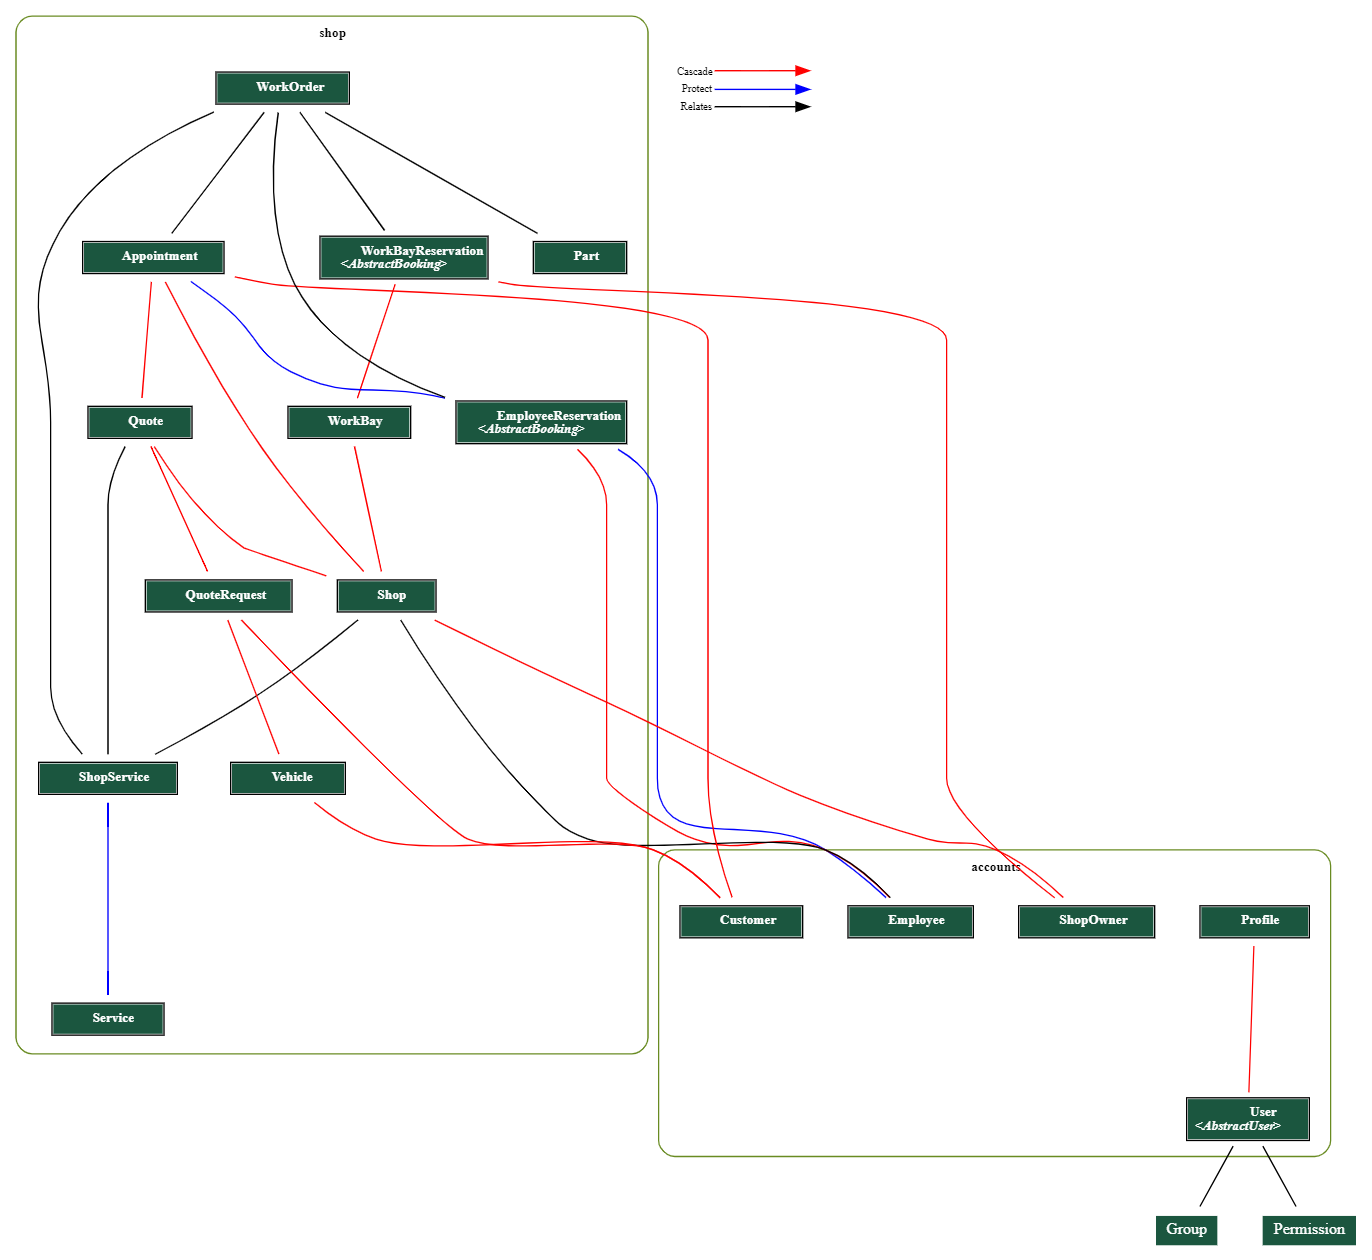
\includegraphics[scale=0.35]{Design/SoftArchitecture/updated-backend-minimal.png}
    \caption{Backend Module Hierarchy Diagram}
    \label{fig:backend-mh}
\end{figure}

\begin{figure}
    \centering
    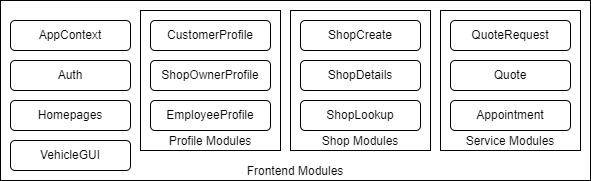
\includegraphics[width=1.0\textwidth]{Design/SoftArchitecture/front_hierarchy.png}
    \caption{Frontend Module Hierarchy Diagram}
    \label{FigUH}
\end{figure}

For a higher resolution diagram check appendix.

% Frontend Module Hierarchy Diagram - Kai

This section provides an overview of the module design. Modules are summarized
in a hierarchy decomposed by secrets in Table \ref{TblMH}. The modules listed
below, which are leaves in the hierarchy tree, are the modules that will
actually be implemented.

\begin{table}[H]
    \centering
    \begin{tabularx}{\textwidth}{XX}
        \textbf{Backend Modules} & \textbf{Frontend Modules} \\ \hline
        \bemoduledef{Profile} & \femoduledef{Auth} \\
        \bemoduledef{Shop} & \femoduledef{Vehicles} \\
        \bemoduledef{ShopService} & \femoduledef{Homepages} \\
        \bemoduledef{Service} & \femoduledef{ShopLookup} \\
        \bemoduledef{EmployeeAvailability} & \femoduledef{CustomerProfile} \\
        \bemoduledef{VehiclesInfo} & \femoduledef{ShopOwnerProfile} \\
        \bemoduledef{Quote} & \femoduledef{EmployeeProfile} \\
        \bemoduledef{QuoteRequest} & \femoduledef{Quote} \\
        \bemoduledef{Appointment} & \femoduledef{QuoteRequest} \\
         & \femoduledef{ShopCreate} \\
        & \femoduledef{ShopDetails} \\
        & \femoduledef{AppContext} \\
        & \femoduledef{Appointment} \\
    \end{tabularx}
    \caption{List of backend and frontend leaf modules}
    \label{TblMH}
\end{table}

\section{Connection Between Requirements and Design} \label{SecConnection}

% Ethan
The design of the system is intended to satisfy the requirements developed in
the SRS. In this stage, the system is decomposed into modules. The connection
between requirements and modules is listed in Table~\ref{TblFRT}.

\begin{itemize}
    \item Several requirements in the SRS (i.e. SR1, PAR11, ApR3, etc.) mention different behaviours of the system based on the class of user (employee, customer, shop owner). For this reason the functionality of profile-related actions such as updating account details and changing shop/personal availability have been split on the frontend into multiple class specific modules. This allows for logic across the same user class to be fully encapsulated and easily modified in the future, while maintaining a simple backend architecture.
    \item A large amount of non-functional requirements for \progname{} specify visual design preferences and usability goals intended to be enforced across the entire system. To achieve this level of consistency and simplify the frontend design process, a framework like React Bootstrap will be used as these components already meet the required design characteristics of the system.
\end{itemize}

\section{Module Decomposition} \label{SecMD}
% Backend
%   shop
    %   Quotes - Alyssa 
    %   QuoteRequests - Alyssa
    %   Shop - Chris
    %   ShopService - Chris
    %   Service - Chris
    %   Vehicles - Ethan-
    %   Apppointment - Harsh
    %   Workorders - Harsh
%   accounts
    % Profile - Kai
% Frontend
%   Auth - Kai
%   Profile
    % Customer - Ethan-
        % Vehicles
    % Shop Owner - Ethan-
    % Employee - Ethan-
%   ShopLookup - Collin
%   ShopCreate - Chris
%   Quotes - Alyssa
%   QuoteRequest - Alyssa
%   Homepages - Ethan-
%   Apppointment - Harsh
%   Workorders - Harsh

Modules are decomposed according to the principle of ``information hiding''
proposed by Parnes et al.. The \emph{Secrets} field in a module
decomposition is a brief statement of the design decision hidden by the
module. The \emph{Services} field specifies \emph{what} the module will do
without documenting \emph{how} to do it. For each module, a suggestion for the
implementing software is given under the \emph{Implemented By} title. If the
entry is \emph{OS}, this means that the module is provided by the operating
system or by standard programming language libraries.  \emph{\progname{}} means the
module will be implemented by the \progname{} software.

Only the leaf modules in the hierarchy have to be implemented. If a dash
(\emph{--}) is shown, this means that the module is not a leaf and will not have
to be implemented.

\subsection{Backend Modules}
\subsubsection{Profile module (\beref{beProfile}) \labelbedef{Profile}}
\begin{description}
\item[Secrets:] Holds account profile related information such as name, contact, user type
\item[Services:] Methods to create new accounts, update existing information, and reset passwords
\item[Implemented By:] \progname
\item[Type of Module:] Abstract Data Type
\end{description}

\subsubsection{Shop Module (\beref{beShop}) \labelbedef{Shop}}

\begin{description}
\item[Secrets:] Shop model containing information including name, address, description, email, phone, address, services, employees, and owner account.
\item[Services:] Methods to create, update, read, and delete a Shop instance.
\item[Implemented By:] \progname
\item[Type of Module:] Abstract Data Type
\end{description}

\subsubsection{ShopService Module (\beref{beShopService}) \labelbedef{ShopService}}

\begin{description}
\item[Secrets:] ShopService model containing information including price, estimated time, and service.
\item[Services:] Methods to create, update, read, and delete a ShopService instance.
\item[Implemented By:] \progname
\item[Type of Module:] Abstract Data Type
\end{description}

\subsubsection{Service Module (\beref{beService}) \labelbedef{Service}}

\begin{description}
\item[Secrets:] Service model containing information including name and description.
\item[Services:] Methods to create, update, read, and delete a Service instance.
\item[Implemented By:] \progname
\item[Type of Module:] Abstract Data Type
\end{description}

%\subsubsection{Part Module (\beref{bePart}) \labelbedef{Part}}

%\begin{description}
%\item[Secrets:] Part model.
%\item[Services:] Methods to define a part, its type and price. 
%\item[Implemented By:] \progname
%\item[Type of Module:] Abstract Data Type
%\end{description}

\subsubsection{EmployeeAvailability Module (\beref{beEmployeeAvailability}) \labelbedef{EmployeeAvailability}}

\begin{description}
\item[Secrets:] EmployeeAvailability, EmployeeAvailabilityOccurrence, EmployeeTimeSlot and EmployeeReservation models.
\item[Services:] Methods to access the available availability objects, set up time slots and reservations, and approve or reject a reservation. 
\item[Implemented By:] \progname
\item[Type of Module:] Abstract Data Type
\end{description}

\subsubsection{VehiclesInfo Module (\beref{beVehiclesInfo}) \labelbedef{VehiclesInfo}}
\begin{description}
    \item[Secret:] Characteristic details of vehicle types (make, model, year, etc.)
    \item[Services:] Storage, retrieval and modification of vehicle information
    \item[Implemented By:] \progname
    \item[Type of Module:] Record
\end{description}

\subsubsection{Quote Module (\beref{beQuote}) \labelbedef{Quote}}

\begin{description}
\item[Secrets:] The information contained in a quote that is sent to an automotive shop, filled in and sent on the frontend by a customer.
\item[Services:] Defines the information contained in a quote that is displayed to an automotive shop.
\item[Implemented By:] Sayyara
\item[Type of Module:] Abstract Data Type
\end{description}

\subsubsection{QuoteRequest Module (\beref{beQuoteRequest}) \labelbedef{QuoteRequest}}

\begin{description}
\item[Secrets:] The information contained in a quote request that is filled in and sent to automotive shops by customers. This differs from the Quote module as the QuoteRequest module contains additional information relevant to the customer, and contains all shops sent to rather than just one quote per shop.
\item[Services:] Defines the information contained in a quote request, modifiable by the customer.
\item[Implemented By:] Sayyara
\item[Type of Module:] Abstract Data Type
\end{description}

\subsubsection{Appointment Module (\beref{beAppointment}) \labelbedef{Appointment}}

\begin{description}
\item[Secrets:] Appointment model.
\item[Services:] Methods to create an appointment, set the estimated time and price, associate the appointment with a customer and shop, and send a confirmation email.
\item[Implemented By:] \progname
\item[Type of Module:] Record
\end{description}

% \subsubsection{WorkOrder Module (\beref{beWorkOrder}) \labelbedef{WorkOrder}}

% \begin{description}
% \item[Secrets:] Appointment, EmployeeReservation, ShopService, Part, and WorkBayReservation models. 
% \item[Services:] Methods to create a work order, associate it with appointments and reservations, associate services and parts with the work order, and set the status, description, price and note for the work order. 
% \item[Implemented By:] \progname
% \item[Type of Module:] Record
% \end{description}

\subsection{Frontend Modules}

\begin{description}
\item[Secrets:]The contents of the required behaviours.
\item[Services:]Includes programs that provide externally visible behaviour of
  the system as specified in the software requirements specification (SRS)
  documents. This module serves as a communication layer between the
  hardware-hiding module and the software decision module. The programs in this
  module will need to change if there are changes in the SRS.
\item[Implemented By:] --
\end{description}

\subsubsection{Auth Module (\feref{feAuth}) \labelfedef{Auth}}

\begin{description}
\item[Secrets:]Contains authentication status and tokens
\item[Services:]Methods for connecting to backend APIs related to account authentication and registration
\item[Implemented By:] \progname
\item[Type of Module:] Library
\end{description}

\begin{description}
\item[Secrets:] Customer, Shop, Quote, and EmployeeReservation models.
\item[Services:] Methods to create an appointment, set the estimated time and price, and associate the appointment with a customer and shop. 
\item[Implemented By:] \progname
\item[Type of Module:] Record
\end{description}

\subsubsection{Vehicles Module (\feref{feVehicles}) \labelfedef{Vehicles}}
\begin{description}
    \item[Secrets:] Information presented to the user regarding vehicles, and event handling of the vehicles page
    \item[Services:] GUI output containing appropriate information/elements for vehicle management
    \item[Implemented By:] \progname
    \item[Type of Module:] Abstract Object
\end{description}

\subsubsection{Homepages Module (\feref{feHomepages}) \labelfedef{Homepages}}
\begin{description}
    \item[Secrets:] Event handling and GUI output formatting of the website landing page, for all classes of user
    \item[Services:] GUI output containing homepage-related information appropriate for the user type
    \item[Implemented By:] \progname
    \item[Type of Module:] Abstract Object
\end{description}

\subsubsection{ShopLookup Module (\feref{feShopLookup}) \labelfedef{ShopLookup}}

\begin{description}
\item[Secrets:] Shop model
\item[Services:] Provides users with a way to search for a shop by name or postal code. Users can also filter by distance. 
\item[Implemented By:] \progname
\item[Type of Module:] Abstract Object
\end{description}

\subsubsection{CustomerProfile Module (\feref{feCustomerProfile}) \labelfedef{CustomerProfile}}
\begin{description}
    \item[Secrets:] Event handling and GUI output formatting of the customer profile page
    \item[Services:] GUI output containing customer profile related information
    \item[Implemented By:] \progname
    \item[Type of Module:] -
\end{description}

\subsubsection{ShopOwnerProfile Module (\feref{feShopOwnerProfile}) \labelfedef{ShopOwnerProfile}}
\begin{description}
    \item[Secrets:] Event handling and GUI output formatting of the shop owner profile page
    \item[Services:] GUI output containing shop owner profile related information
    \item[Implemented By:] \progname
    \item[Type of Module:] Abstract Object
\end{description}

\subsubsection{EmployeeProfile Module (\feref{feEmployeeProfile}) \labelfedef{EmployeeProfile}}
\begin{description}
    \item[Secrets:] Event handling and GUI output formatting of the employee profile page
    \item[Services:] GUI output containing employee profile related information
    \item[Implemented By:] \progname
    \item[Type of Module:] Abstract Object
\end{description}

\subsubsection{Quote Module (\feref{feQuote}) \labelfedef{Quote}}

\begin{description}
\item[Secrets:] Event handling and GUI output formatting of the shop quote page
\item[Services:] GUI output containing shop quote related information. The shop employee is able to view and respond to new quote requests submitted by customers and can view the history of all quotes for said shop.
\item[Implemented By:] \progname
\item[Type of Module:] Abstract Object
\end{description}

\subsubsection{QuoteRequest Module (\feref{feQuoteRequest}) \labelfedef{QuoteRequest}}

\begin{description}
\item[Secrets:] Event handling and GUI output formatting of the customer quote request page
\item[Services:] GUI output containing customer quote request related information. The customer is also able to fill out new quote requests, and edit or delete existing quote requests.
\item[Implemented By:] \progname
\item[Type of Module:] Abstract Object
\end{description}

\subsubsection{ShopCreate Module (\feref{feShopCreate}) \labelfedef{ShopCreate}}

\begin{description}
    \item[Secrets:] Event handling and GUI output formatting of the ShopCreate page
    \item[Services:] GUI output containing fields for the shop owner to fill in and create their Shop instance in the backend
    \item[Implemented By:] \progname
    \item[Type of Module:] Abstract Object
\end{description}

\subsubsection{ShopDetails Module (\feref{feShopDetails}) \labelfedef{ShopDetails}}

\begin{description}
\item[Secrets:] Shop Service, and Service models.
\item[Services:] Provides customer with the types of services a certain shop may offer.
\item[Implemented By:] \progname
\item[Type of Module:] Abstract Object
\end{description}

\subsubsection{AppContext Module (\feref{feAppContext}) \labelfedef{AppContext}}
\begin{description}
\item[Secrets:]Holds application-level states including authentication
\item[Services:]Methods for setting application-level variables
\item[Implemented By:] \progname
\item[Type of Module:] Abstract Object
\end{description}

\subsubsection{Appointment Module (\feref{feAppointment}) \labelfedef{Appointment}}

\begin{description}
\item[Secrets:] Appointment model.
\item[Services:] Methods to create an appointment, set the estimated time and price, and associate the appointment with a customer and shop.  
\item[Implemented By:] \progname
\item[Type of Module:] Abstract Object
\end{description}


% \subsubsection{WorkOrder Module (\feref{feWorkOrder}) \labelfedef{WorkOrder}}

% \begin{description}
% \item[Secrets:] WorkOrder model.
% \item[Services:] Methods to create a work order, set the estimated time and price, and associate the work order with an appointment, employee reservation, shop service, part, and work bay reservation. 
% \item[Implemented By:] \progname
% \item[Type of Module:] Abstract Object 
% \end{description}

\newpage

\section{Traceability Matrix} \label{SecTM}

This section shows two traceability matrices: between the modules and the functional
requirements and the modules and the anticipated changes.

% the table should use mref, the requirements should be named, use something
% like fref
\begin{table}[H]
\centering
\begin{tabular}{p{0.1\textwidth} p{0.6\textwidth}}
\toprule
\textbf{Req.} & \textbf{Modules}\\
\midrule
AuR1 & \beref{beProfile}, \feref{feAuth}, \feref{feAppContext} \\
AuR2 & \beref{beProfile}, \feref{feAuth}, \feref{feAppContext} \\
AuR3 & \beref{beProfile}, \feref{feAuth} \\
SR1 & \beref{beShop}, \beref{beShopService}, \feref{feShopOwnerProfile}, \feref{feShopCreate}\\
SR2 & \beref{beShop}, \beref{beShopService}, \feref{feShopLookup}, \feref{feShopDetails}, \feref{feShopOwnerProfile} \\
PAR1 & \beref{beShop}, \feref{feShopOwnerProfile} \\
PAR2 & \beref{beShop}, \feref{feShopOwnerProfile} \\
PAR3 & \beref{beProfile}, \feref{feCustomerProfile}, \feref{feShopOwnerProfile}, \feref{feEmployeeProfile} \\
PAR4 & \beref{beShop}, \feref{feShopLookup}, \feref{feShopDetails} \\
PAR5 & \beref{beShop}, \feref{feShopOwnerProfile} \\
PAR6 & \beref{beEmployeeAvailability}, \feref{feShopDetails}, \feref{feShopOwnerProfile}\\
PAR7 & \beref{beProfile}, \feref{feShopOwnerProfile} \\
PAR8 & \beref{beProfile}, \feref{feShopOwnerProfile} \\
% PAR9 & \beref{beProfile}, \feref{feShopOwnerProfile}, \feref{feShopCreate} \\
PAR9 & \beref{beProfile}, \feref{feAuth}, \feref{feEmployeeProfile} \\
PAR10 & \feref{feEmployeeProfile} \\
ApR1 & \beref{beShop}, \beref{beEmployeeAvailability}, \feref{feShopOwnerProfile} \\
ApR2 & \beref{beQuote}, \beref{beQuoteRequest}, \beref{beAppointment}, \feref{feQuote}, \feref{feQuoteRequest} \\
ApR3 & \beref{beQuote}, \beref{beQuoteRequest}, \beref{beAppointment}, \feref{feQuote}, \feref{feQuoteRequest} \\
ApR4 & \beref{beQuoteRequest}, \feref{feQuoteRequest} \\
% WOR1 & \beref{beWorkOrder}, \feref{feWorkOrder} \\
% WOR2 & \beref{beWorkOrder}, \feref{feWorkOrder} \\
% WOR3 & \beref{beAppointment}, \beref{beWorkOrder}, \feref{feWorkOrder} \\
QR1 & \beref{beQuote}, \beref{beQuoteRequest}, \feref{feQuote}, \feref{feQuoteRequest} \\
QR2 & \feref{feQuoteRequest} \\
QR3 & \beref{beQuote}, \beref{beQuoteRequest}, \feref{feQuote}, \feref{feQuoteRequest} \\
%VR1 & \beref{bePart} \\
%VR2 & \beref{bePart} \\
\bottomrule
\end{tabular}
\caption{Trace Between Functional Requirements and Modules}
\label{TblFRT}
\end{table}

\begin{table}[H]
\centering
\begin{tabular}{p{0.2\textwidth} p{0.6\textwidth}}
\toprule
\textbf{AC} & \textbf{Modules}\\
\midrule
\hyperref[acDevice]{AC1} & \feref{feAuth}, \feref{feVehicles}, \feref{feHomepages}, \feref{feShopLookup}, \feref{feShopDetails}, \feref{feCustomerProfile}, \feref{feShopOwnerProfile}, \feref{feEmployeeProfile}, \feref{feQuote}, \feref{feQuoteRequest}, \feref{feShopCreate} \feref{feAppContext}, \feref{feAppointment}, \feref{feWorkOrder}\\
\hyperref[acUsers]{AC2} & \beref{beProfile} \\
\hyperref[acStorage]{AC3} & \beref{beProfile}, \beref{beShop}, \beref{beShopService}, \beref{beService}, \beref{beEmployeeAvailability}, \beref{beVehiclesInfo}, \beref{beQuote}, \beref{beQuoteRequest}, \beref{beAppointment}, \beref{beWorkOrder}\\
\hyperref[acBandwidth]{AC4} & \beref{beProfile}, \beref{beShop}, \beref{beShopService}, \beref{beService}, \beref{beEmployeeAvailability}, \beref{beVehiclesInfo}, \beref{beQuote}, \beref{beQuoteRequest}, \beref{beAppointment}, \beref{beWorkOrder}\\
\hyperref[acGUI]{AC5} & \feref{feAuth}, \feref{feVehicles}, \feref{feHomepages}, \feref{feShopLookup}, \feref{feShopDetails}, \feref{feCustomerProfile}, \feref{feShopOwnerProfile}, \feref{feEmployeeProfile}, \feref{feQuote}, \feref{feQuoteRequest}, \feref{feShopCreate} \feref{feAppContext}, \feref{feAppointment}, \feref{feWorkOrder}\\
\hyperref[acAuth]{AC6} & \feref{feAuth}, \feref{feAppContext} \\
\hyperref[acScheduling]{AC7} & \beref{beAppointment}, \feref{feAppointment} \\
\hyperref[acNotification]{AC8} & \beref{beEmployeeAvailability}, \beref{beQuote}, \beref{beQuoteRequest}, \beref{beAppointment}, \beref{beWorkOrder} \\
\hyperref[acHardware]{AC9} & \beref{beProfile}, \beref{beShop}, \beref{beShopService}, \beref{beService}, \beref{beEmployeeAvailability}, \beref{beVehiclesInfo}, \beref{beQuote}, \beref{beQuoteRequest}, \beref{beAppointment}, \beref{beWorkOrder}\\
\bottomrule
\end{tabular}
\caption{Trace Between Anticipated Changes and Modules}
\label{TblACT}
\end{table}

\section{Use Hierarchy Between Modules} \label{SecUse}
% Chris - DAG for module-use heirarchy


\begin{figure}[H]
\centering
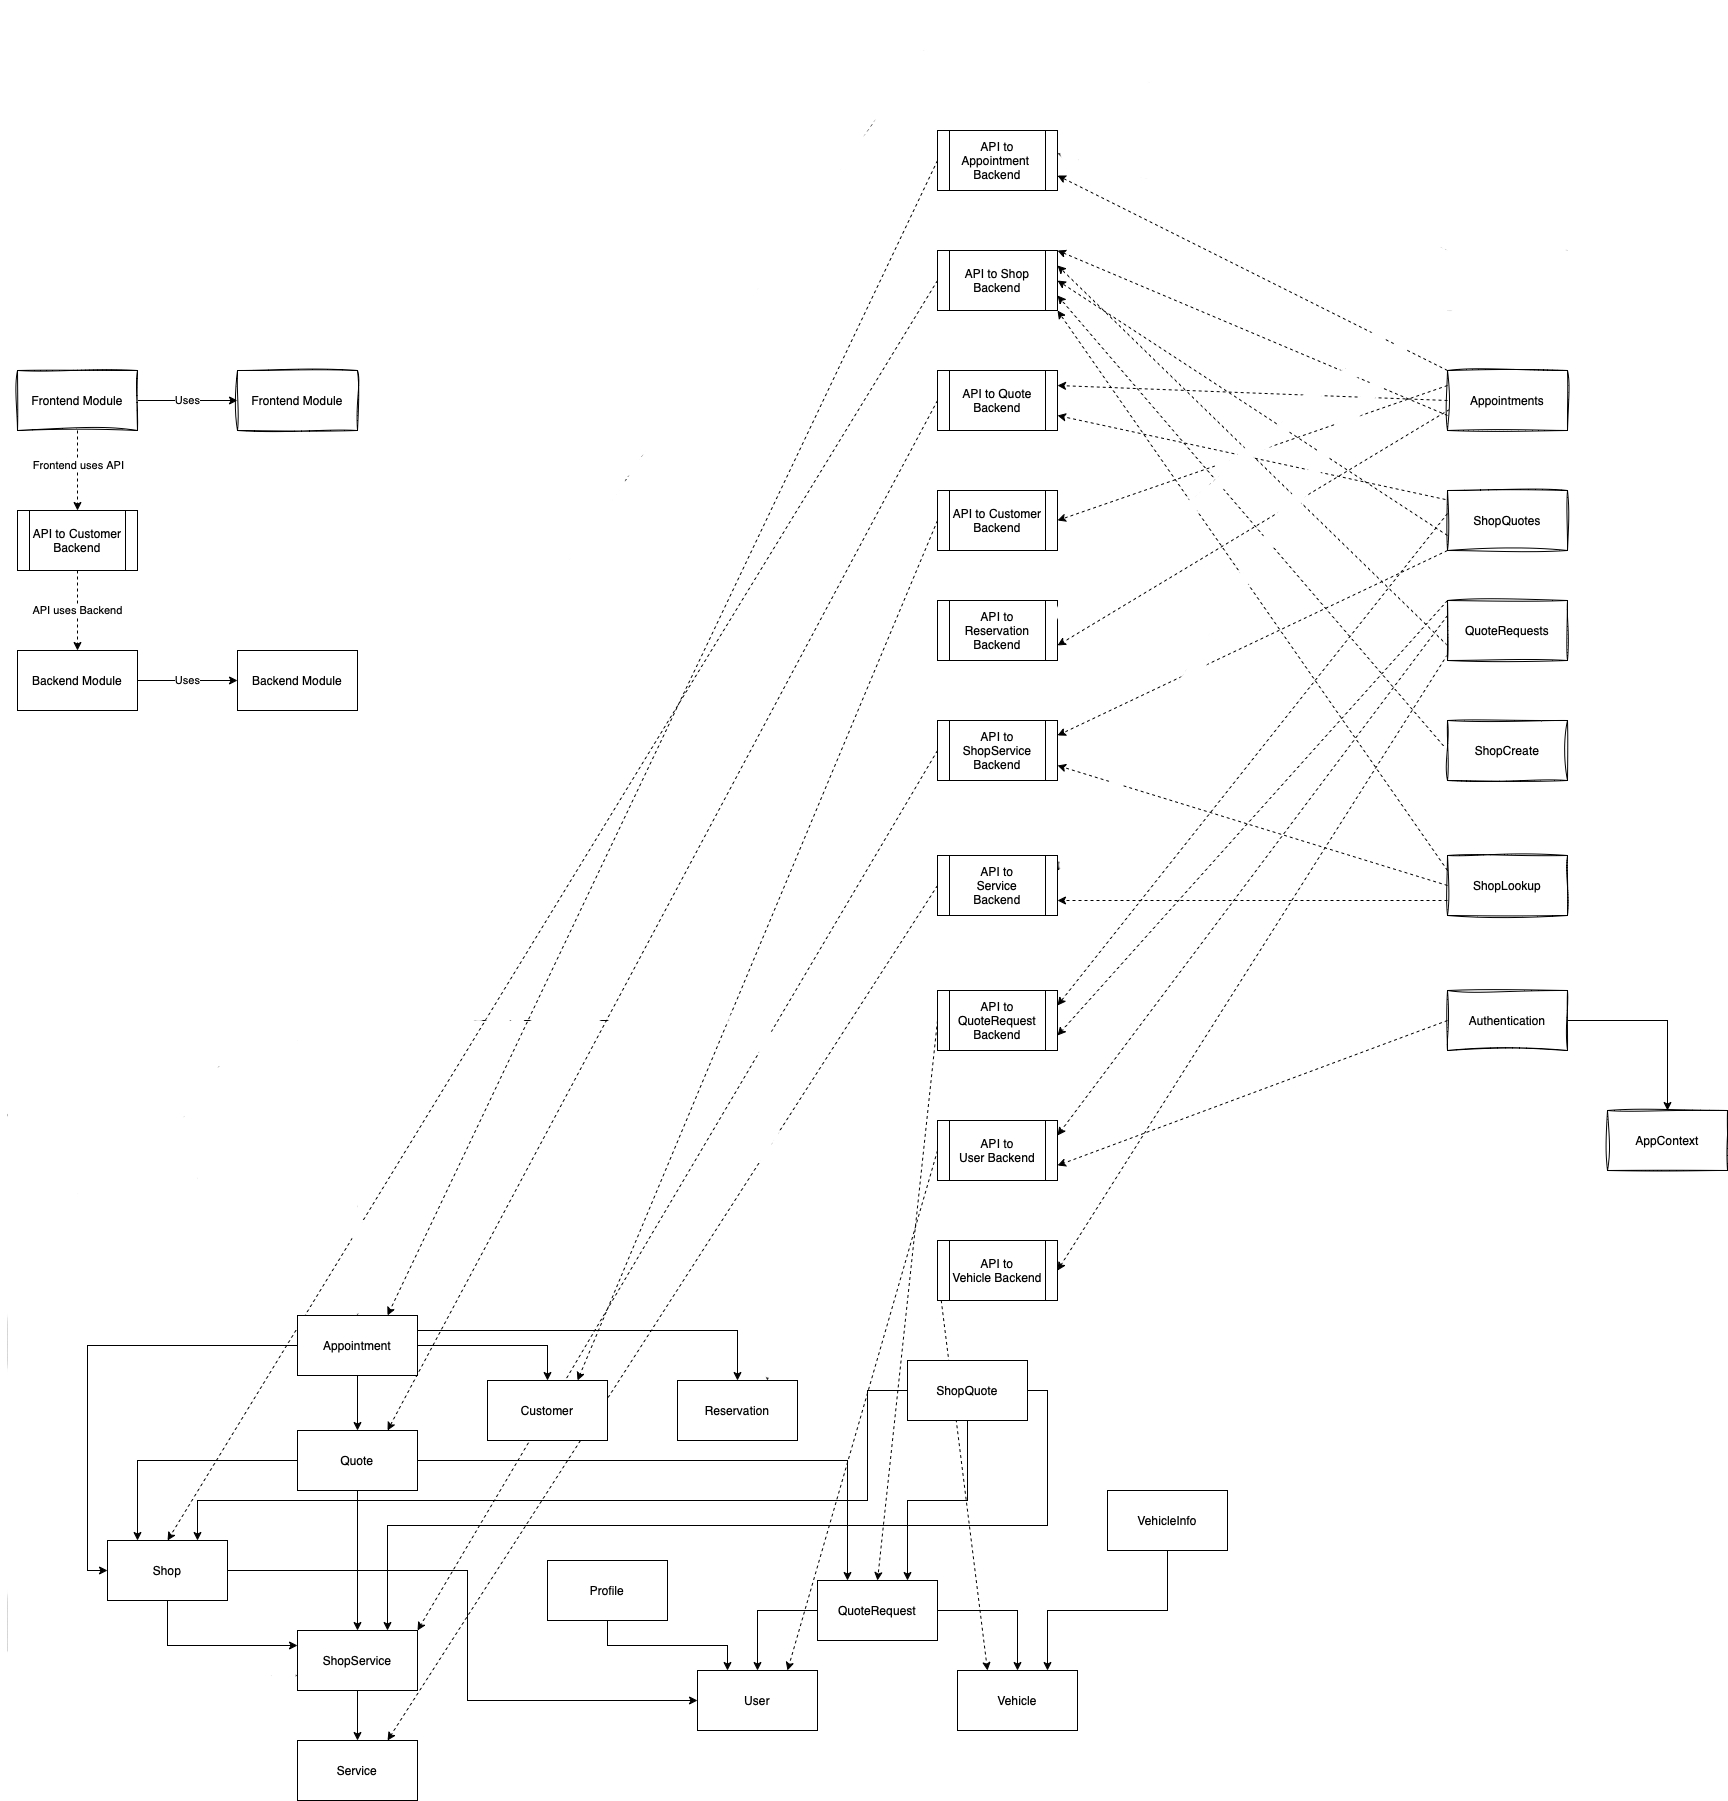
\includegraphics[width=1\textwidth]{use_heirarchy.png}
\caption{Use hierarchy among modules}
\label{FigUH}
\end{figure}

%\section*{References}

\bibliographystyle {plainnat}
\bibliography{../../../refs/References}

\newpage{}

\end{document}